\section{Experimental Evaluation}

We report the experimental result of running three benchmark queries from 
Section~\ref{sec:benchmark}. We deployed the three systems in Amazon EC2 using 
the identical configuration, which uses 1 master node and 16 slave nodes.
Each node is a m3.large instance which has 2 vCPU, 7.5 GB RAM and 32GB SSD 
storage. We used the most up to date version of the 3 systems that we can get:
Myria (Daily built in Mar 10, 2015, commit: 90d85cd), Spark (1.2.1 release) and
GraphLab (Open sourced version in GitHub, commit: 18c2103). All our source code
is open sourced in \url{https://github.com/stechu/CSE544_Project}.

\subsection{Objective Evaluation}
\label{subsec:obje}

\subsubsection{Q1}

We evaluate the performance of three systems on Q1 using jstor scientific digital
library data. We use two tables: 
\begin{enumerate}
    \item Paper(pid:int, year:int) is a table with two columns. The first column is the unique paper id of each paper. The second column is the year
    when the paper was published. This table contains 1.8 million papers.
    \item Citation(p1:int, p2:int) is a table with two columns. Each row of 
    this paper represents a citation. The first column of this table is the
    citing paper, and the second is the cited paper. This table contains 8.2
    million citations.
\end{enumerate}

Figure~\ref{fig:q1} shows the runtime and lines of code (LOC) using three 
systems. We can observe the GraphLab has the fastest runtime among three 
systems. Myria is slightly slower (1.38x runtime) than GraphLab. Spark is 
slowest among the three systems. Its runtime is 43x GraphLab's runtime.  
In term of LOC (Figure~\ref{fig:q1_loc}), both Myria and Spark use less than 
70 lines to express this query while GraphLab need nearly 400 lines. This is 
due to the programming model and the language support. GraphLab uses C++ and 
force the programmer to ``think like a vertex''.

\begin{figure}[t]
    \centering
    \begin{subfigure}{0.7\linewidth}
        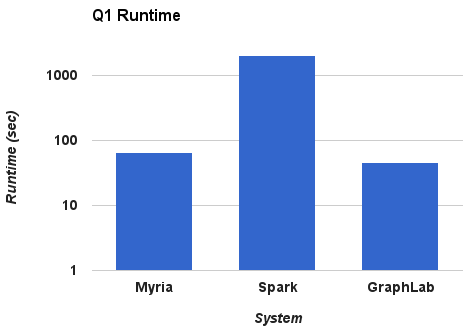
\includegraphics[width=\textwidth]{images/q1_runtime.png}
        \caption{Runtime}
        \label{fig:q1_runtime}
    \end{subfigure}
    \begin{subfigure}{0.7\linewidth}
        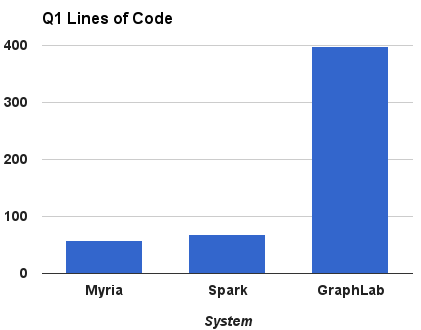
\includegraphics[width=\textwidth]{images/q1_loc.png}
        \caption{Lines of Code}
        \label{fig:q1_loc}
    \end{subfigure}
\caption{Q1: LCA}
\label{fig:q1}
\end{figure}

\subsubsection{Q2}

We evaluate the performance of the three system on Q2 using sampled twitter 
social network data. The table contains two columns, the first column is the 
id of follower and the second is the id of the followee. Since $k$-core
requires a undirected graph, we add an reversed edge between two nodes 
if there is a single directed edge between them. The tables contains about 
2 million rows.

Figure~\ref{fig:q2} shows the runtime and lines of code using three systems. 
We can observe that Myria has smallest runtime among all the three systems. 
GraphLab has about $1.8x$ Myria's runtime and Spark has about $5x$ Myria's 
runtime. In terms of lines of code, Myria needs only $13$ lines of code, while
Spark needs $23$ lines of code and GraphLab used $146$ lines of code. 

\begin{figure}[t]
    \centering
    \begin{subfigure}{0.7\linewidth}
        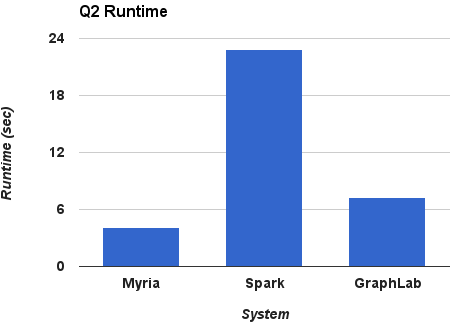
\includegraphics[width=\textwidth]{images/q2_runtime.png}
        \caption{Runtime}
        \label{fig:q2_runtime}
    \end{subfigure}
    \begin{subfigure}{0.7\linewidth}
        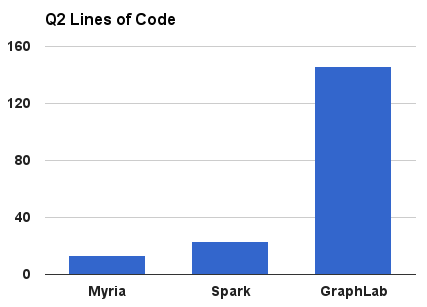
\includegraphics[width=\textwidth]{images/q2_loc.png}
        \caption{Lines of Code}
        \label{fig:q2_loc}
    \end{subfigure}
\caption{Q2: k-core}
\label{fig:q2}
\end{figure}

\subsubsection{Q3}

We evaluate the performance of the three systems on Q3 using $13$ snapshots of 
galaxy data from UW astronomy department. We use two tables:

\begin{enumerate}
    \item Halo(grpId:long, timeStep:long, mass:double, numParticles: long) is 
    a table with 4 columns. The first two columns form a unique identification 
    (primary key) for a halo. The third column is the mass of a halo. The
    forth column contains the number of particles within a halo. This table 
    contains 68K halos.
    \item ParticleOfInterest(pid:long, mass:double, type:string, grpId:long, 
     timeStep: long) is a table with 5 columns. The first column is the unique
     identifier (primary key) of a particle. The second column is the mass of a
     particle. The third column contains the type of a particle. The last two 
     columns decides which group (halo) a particle belongs to. This table
     contains 42 million particles.
\end{enumerate}

XXXXXXXXXXXXXXXXXXXXXXXXXXXXXXXXXXXXXXXX

ADD PERFORMANCE AND LOC COMPARISON HERE

XXXXXXXXXXXXXXXXXXXXXXXXXXXXXXXXXXXXXXXX

\begin{figure}[t]
    \centering
    \begin{subfigure}{0.7\linewidth}
        Q3 RUNTIME FIGURE HERE
        \caption{Runtime}
        \label{fig:q3_runtime}
    \end{subfigure}
    \begin{subfigure}{0.7\linewidth}
        Q3 LOC FIGURE HERE
        \caption{Lines of Code}
        \label{fig:q3_loc}
    \end{subfigure}
\caption{Q3: merger tree}
\end{figure}

\subsection{Comparing the three systems}

We try to draw some subjective conclusions for 
the three system from the objective evaluation 
in Section~\ref{subsec:obje} and from our experience of using these three systems in this section.

\subsubsection{Myria}
Myria topped two queries in runtime and topped all three query in LOC, which
clearly shows that on the scenario that we defined. Myria is fast and at a 
very high level of abstraction to make the users who writes analytic queries
easier. We think this good performance comes from two reasons:

\begin{enumerate}
    \item The relational abstraction fits well with ``Big Data''. The 
    relational data model provide user a declarative language that easy 
    to express analytic workload. On the other hand, extensive research
    on query optimization will enable efficient parallel evaluation of 
    the relational query.
    \item As a state of art distributed shared nothing database system, 
    Myria adopted many new technology such as light weight iterative 
    processing and parallel data flow based back-end engine. The good 
    system implementation contributes to the performance as well. 
\end{enumerate} 

The inconvenience of using Myria is its data ingestion process. Although the 
system support ingesting data from S3, the user have to use post a json 
formatted query to do the data ingestion while cannot direct write S3 bucket 
as the data source in the query.

\subsubsection{Spark}

Spark is a new MapReduce implementation with significant improvement on 
iterative and in-memory computing ability. We find that the most significant  
strengths of spark is its
Well matured and system and eco-system. Spark is very easy to
deploy in EC2. The programming guide and documentation is very user friendly. 

In terms of abstraction level, Spark is below Myria. In Spark python, user 
still need to use MapReduce like transform function to operate data. It is 
slightly less convenient compared with Myria. For example, to do a join, the 
the user need firstly apply a map with a function which transform the joined 
columns to key. But overall, using Spark python to express all the three query
is not hard and uses relatively small LOCs.

The biggest problem of Spark is performance. Spark is the slowest system in 2 
of 3 queries. We do not have a concrete idea on the reason for that. But our 
guess could be the synchronization barrier over iteration in spark is still 
larger than other modern systems (Myria and GraphLab), although improved 
largely from Hadoop MapReduce.

Another problem of Spark is lacking automatic control of parallelism of RDD. 
The parallelism of RDD will be the sum of the two source RDDs if user joins
them. This causes the parallelism of RDD grows exponentially if there are
joins inside an iteration. This will quickly lead to run out of system 
sources since the overhead of each RDD container is not negligible. This 
problem can be solved by forcing keeping parallelism after join. But it is
not very easy for a user to identify this problem and find the solution.   
    
\subsubsection{GraphLab}

XXXXXXXXXXXXXXXXXXXXXXXXXX
TO BE COMPLETED BY EDWARD
XXXXXXXXXXXXXXXXXXXXXXXXXX